\subsection{\ugrid{} Topolgy}
An unstructured (\ugrid{}) topology is defined as a topology that is
not regular, i.e., does not admit a closed-form representation of
sample locations and connectivity. Unstructured topologies offer the
highest level of flexibility from a visualization and modeling
standpoint as higher sampling frequencies may be used in regions of
interest while sparsely sampling low-impact areas to conserve
computational resources. As such, many modern \cf{} prediction and
modeling algorithms compute attributes associated with unstructured
topologies.

Historically, there is a large quantity of \cf{} data associated with
structured topologies. As storage and processing hardware has become
more accessible, complex unstructured representations have become more
prevalent. However, most existing visualization technologies in the
\cf{} community can render only simpler, structured
datasets. \sciwms{} is one of the first visualization services to
support rendering data with unstructured topologies.

Any NCML file exposing the topology of an externally hosted
dataset according to the \cfugrid{} sepcification can be processed by
\sciwms{}. According the \cfugrid{} standard, a topology is always
embedded on the real line, in the plane or space with sample
locations, the vertices of the topology, exposed as an array of
coordinates in the appropriate ambient space. Vertex connectivity is
expressed as a $M \times D$ array where each element is an index into
the vertex list. The dimension of a topology (equal to $D - 1$) defines the
atomic spatial element created by the connectivity list. In \cfugrid{}
terminology, a topology with dimension 0 defines a set of disconnected
points (no connectivity) called \textbf{\textit{nodes}}, a 1D topology
consists of lines or curved boundaries known as
\textbf{\textit{edges}}, a 2D topology is a set of planes or surfaces
enclosed by a set of edges (e.g. triangulation) called
\textbf{\textit{faces}}, and a 3D topology specifies the volume enclosed
by a set of faces called \textbf{\textit{volumes}}.
For example, figure~\ref{fig:xytable} visualizes a list of a sample
locations as an array of coordinates in the real plane. Topology
connectivity is specified by a list of indicies into the vertex array
interpreted anticlockwise. 

%% Figure~\ref{fig:vtable} visualizes a 2D
%% connectivity list, defining a triangulation in the plane, for the
%% vertex array in figure~\ref{fig:xytable} where each entry indexes an
%% element of the vertex list: $v_n^{\cdot}\in \{0,\ldots,N-1\}$. Each
%% row of the connectivity array defines a triangle: triangle $m$ is
%% specified by linking the coordinates associated with vertex lists by
%% connecting $v^0_m$ to $v^1_m$ to $v^2_m$ and back to $v^0_m$.
%% \begin{figure}[ht!]
%%   \centering
%%   \begin{subfigure}[t]{0.33\textwidth}
%%     \centering
%%     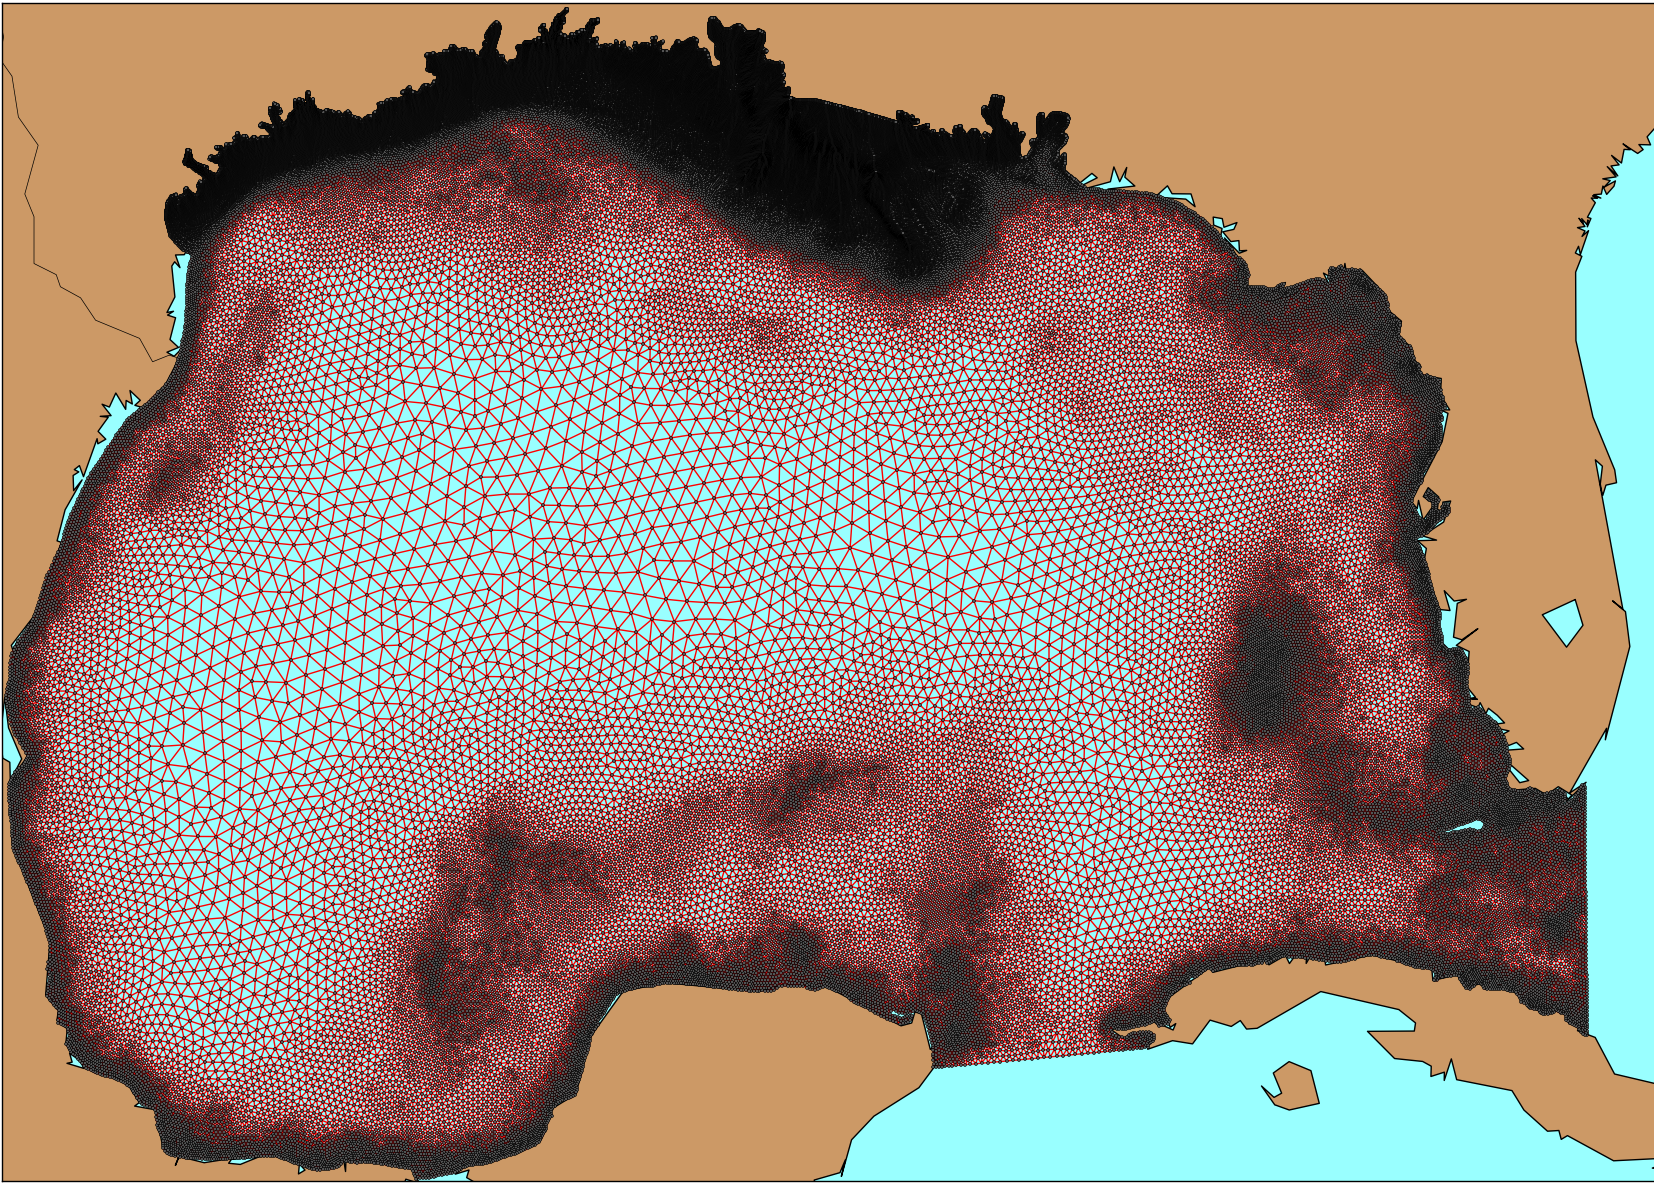
\includegraphics[height=1.3in]{../figs/USF_FVCOM_Hurricane_Ike_2D_final_run_with_waves_topology.png}
%%     \caption{}
%%     \label{fig:usf_fvcom_ugrid}
%%   \end{subfigure}
%%   \begin{subfigure}[t]{0.32\textwidth}
%%     \centering
%%     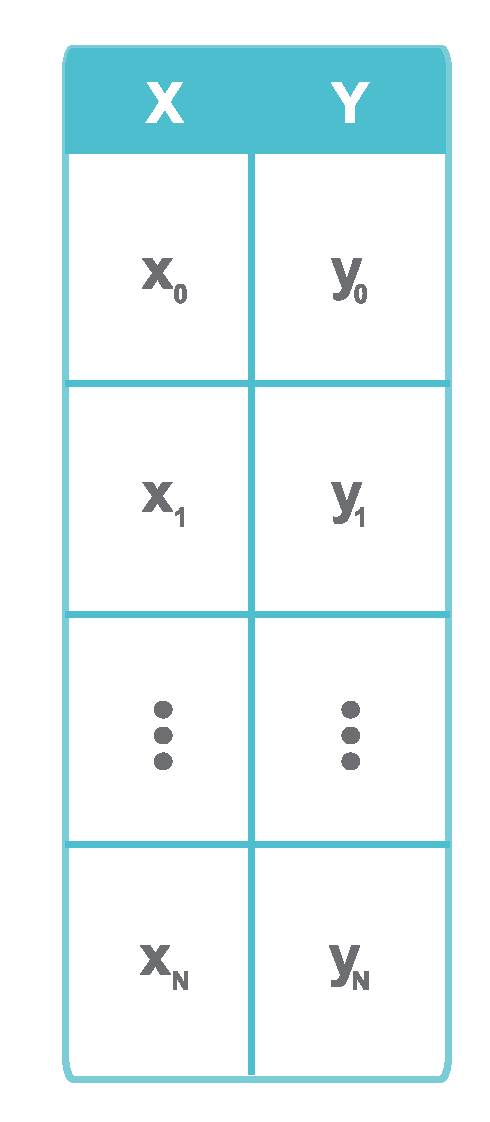
\includegraphics[height=1.35in]{../figs/xy_table}
%%     \caption{}
%%     \label{fig:xytable}
%%   \end{subfigure}
%%   \begin{subfigure}[t]{0.32\textwidth}
%%     \centering
%%     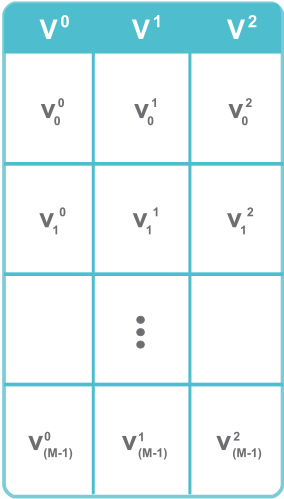
\includegraphics[height=1.35in]{../figs/v_table}
%%     \caption{}
%%     \label{fig:vtable}
%%   \end{subfigure}
%%   \caption{Examples of an \ugrid{} topology and \cfugrid compliant
%%     vertex and connectivity arrays. (a) The location of $N$
%%     vertices in the real plane. (b) A 2D topology with
%%     $M$ triangles. Each triangle represented as a row in the table
%%     referencing locations as indices into the vertex array.}
%% \end{figure}

%% Figure~\ref{fig:usf_fvcom_ugrid} shows a \ugrid{} 2D topology, a
%% triangulation in the plane, used by a climate model for simulating
%% hurricane conditions in the Gulf of Mexico. Vertices represent
%% locations where attributes are estimated and the connectivity is shown
%% as red lines connecting the vertices throughout the region of
%% interest. The visualization was produced by accessing the \cfugrid{}
%% compliant \ncml{} file.
The \ugrid{} topology allows the modelers to save storage and
computational resources by sparsely sampling areas where accuracy can
be sacrificed, such as the center of the Gulf, while allowing for
higher sampling rates where accuracy is paramount, such as densely
populated coastal areas. However, \ugrid{} topologies require explicit
enumeration of sample locations and connectivity, requiring
spatially-aware data structures for optimal storage and processing for
performant visualization algorithms. To this end, \sciwms{} maintains
a local topology cache, storing \ugrid{} topologies as
\rtree{}~\cite{Guttman84} data structures on disk local to the
deployment server for fast access along with the connectivity
array. The \rtree{} is created when the dataset is first registered
with the \sciwms{} service. If a change in the underlying data is
detected at an endpoint associated with a topology cache, the \rtree{}
is rebuilt.
